\newpage
\section{Catalyst Saturation}

The model developed up until now considers the situation where the urea-dosing is such that the catalyst neither
saturated nor empty. The ideal case which is also an assumption in the linearized CSTR model. The dynamic model for
catalyst's surface concentration, when considering the saturation and zero concentration limit will be
($\gamma_{proc}(k)$ is defined in \ref{eqn::gamma_proc}):
%=====
\begin{align}
        \sigma^{ub}(k) &= \sigma (k-1) \gamma_{proc}(k-1) + t_s \Gamma k_{ads}(k-1) \con{NH_3}^{in}(k-1)
        \label{eqn::unbounded_sigma_mdl}\\
        \sigma(k) &= \begin{cases}
                                \sigma^{ub}(k) & \text{if }  0 \leq \sigma^{ub}(k) \leq \Gamma\\
                                \Gamma         & \text{if }  \sigma^{ub}(k) > \Gamma \\
                                0              & \text{if }  \sigma^{ub}(k) < 0
                        \end{cases}
        \label{eqn::actual_sigma_mdl}
\end{align}

Thus substituting equation \ref{eqn::sigma_elim} into above equations \ref{eqn::unbounded_sigma_mdl} and \ref{eqn::actual_sigma_mdl}:
%===
\begin{align}
        \sigma^{ub}(k) &= \lrf{\frac{\eta(k)}{\tau(k-1) k_{s2v} k_{scr}(k-1) u_1(k-1)}} \gamma_{proc}(k-1) + t_s \Gamma k_{ads}(k-1) \con{NH_3}^{in}(k-1)\\
        % ====
        \frac{\eta(k+1)}{\tau(k) k_{s2v} k_{scr}(k) u_1(k)} &=
        \begin{cases}
                                \sigma^{ub}(k)     & \text{if }  0 \leq \sigma^{ub}(k) \leq \Gamma\\
                                \Gamma             & \text{if }  \sigma^{ub}(k) > \Gamma \\
                                0                  & \text{if }  \sigma^{ub}(k) < 0
        \end{cases} \\
        % =====
        \implies \eta(k+1) &=
        \begin{cases}
        \lrf{\tau(k) k_{s2v} k_{scr}(k) u_1(k)}\sigma^{ub}(k)         & \text{if }
                0 \leq \sigma^{ub}(k) \leq \Gamma\\
        \lrf{\tau(k) k_{s2v} k_{scr}(k) u_1(k)} \Gamma                & \text{if }
                \sigma^{ub}(k) > \Gamma \\
        0                                                             & \text{if }
                \sigma^{ub}(k) < 0
        \end{cases}
        \label{eqn::eta_cases}
\end{align}
%====
From, the derivation and the parametrization in the last section, specifically, equations \ref{eqn::eta_parm} and
\ref{eqn::phi_NOx}:
\begin{align}
        \lrf{\tau(k) k_{s2v} k_{scr}(k) u_1(k)}\sigma^{ub}(k) &=
        \eta(k) \lrb{\frac{u_1(k)}{F(k)}} \lrb{\frac{F(k-1)}{u_1(k-1)}}
        +\lrb{\frac{u_1(k)}{F(k)}} \pmb \phi_{NO_x}^T \pmb \theta_{NO_x}
        \label{eqn::sigma_ub_param}
\end{align}
%===
Similarly, the second case can be parametrized using the same set of approximations ($Ai$'s) and models of physical quantities (\ref{eqn::residence_time_mdl}, \ref{eqn::k_mdl}),
\begin{align*}
        \lrf{\tau(k) k_{s2v} k_{scr}(k) u_1(k)} \Gamma  &= \frac{\tau_0}{F(k)} \times k_{s2v} \times \pmb \phi(k)^T \pmb \theta_{scr} \times u_1(k) \times \Gamma\\
        % ==
        &= \lrf{\lrb{\frac{u_1(k)}{F(k)}} \pmb \phi^T(k) } \lrf{\Gamma \tau_0 k_{s2v} \pmb \theta_{scr}}
\end{align*}
\begin{align}
        Let, \qquad  \Gamma \tau_0 k_{s2v} \pmb \theta_{scr} &= \pmb \theta_{\Gamma scr}\\
        \lrf{\tau(k) k_{s2v} k_{scr}(k) u_1(k)} \Gamma  &=
        \lrb{\frac{u_1(k)}{F(k)}} \pmb \phi^T(k)  \pmb \theta_{\Gamma scr}
        \label{eqn::gamma_scr}
\end{align}
%===
The conditions for case switching can also be parametrized to the same expressions as (\ref{eqn::sigma_ub_param}) and (\ref{eqn::gamma_scr}) by multiplying both sides of the inequalities by $\lrf{\tau(k) k_{s2v} k_{scr}(k) u_1(k)} (>0)$ which is always positive.

Let,
\begin{align}
        f_{\sigma}(k) &= \eta(k) \lrb{\frac{u_1(k)}{F(k)}} \lrb{\frac{F(k-1)}{u_1(k-1)}}
        +\lrb{\frac{u_1(k)}{F(k)}} \pmb \phi_{NO_x}^T \pmb \theta_{NO_x}\\
        %===
        f_{\Gamma}(k) &= \lrb{\frac{u_1(k)}{F(k)}} \pmb \phi^T(k)  \pmb \theta_{\Gamma scr}
\end{align}

Substituting the above parametrization into equation (\ref{eqn::eta_cases}):
%===
\begin{align}
        \eta(k+1) &=
        \begin{cases}
                f_{\sigma}(k) & \text{if } 0 \leq f_{\sigma}(k) \leq f_{\Gamma}(k)\\
                f_{\Gamma}(k) & \text{if } f_{\sigma}(k) > f_{\Gamma}(k) \\
                0             & \text{if } f_{\sigma}(k) < 0
        \end{cases}
        \label{eqn::eta_cases}
\end{align}
The above cases can be written in min-max form as follows:
\begin{align}
        \eta\lr{k + 1} &= \max \lrf{ 0, \min \lrf{f_{\sigma}(k), f_{\Gamma}(k)}}
        \label{eqn::eta_max_min}
\end{align}
Thus, the $NO_x$ reduction dynamics are bounded by:
\begin{align}
        0 \leq \eta(k+1) \leq f_\Gamma(k)
\end{align}
% ====
The above equation can be interpreted as follows: $\eta$ at any given time step is bounded by the change in concentration due to $NO_x$ reduction when the catalyst is saturated $\lr{\eta_{sat}}$ under the same conditions of flow-rate and inlet $NO_x$ concentration. This relationship can be used to find the optimal values of the parameter $\pmb \theta_{\Gamma scr}$ by solving the following constrained linear programming problem:
\begin{align*}
        \text{Minimize:}& \qquad    \lrb{ \sum_{k = 0}^{N-2} \lrb{\frac{u_1(k)}{F(k)}} \pmb \phi^T(k) } \pmb \theta_{\Gamma scr}\\
        \text{Subject to:}& \qquad
                \bm{\lrb{\frac{u_1(0)}{F(0)}} \pmb \phi^T(0) \\
                    \lrb{\frac{u_1(1)}{F(1)}} \pmb \phi^T(1) \\
                    \vdots \\
                    \lrb{\frac{u_1(N-2)}{F(N-2)}} \pmb \phi^T(N-2) \\
                }
                \pmb \theta_{\Gamma scr}
                \geq
                \bm{\eta(1) \\
                    \eta(2)\\
                    \vdots \\
                    \eta(N-1)}
\end{align*}
\begin{align}
        \label{eqn::optimization_prob}
\end{align}
Effectively we are minimizing the area under the curve of the parametrized saturated system dynamics under the
constraints of the actual system dynamics. This results in the tightly upper bound curve that describes the dynamics of
the system which is always saturated.

It has to be noted that the upper bound of the actual change in concentration due to $NO_x$ reduction $(\eta(k))$ is the inlet concentration of $NO_x$ $(u_1(k-1))$.

%===
Writing the equation (\ref{eqn::eta_max_min}) in terms of the tail-pipe $NO_x$ concentration,
\begin{align}
        x_1(k+1) &= \max \lrf{0, u_1(k) - \max \lrf{ 0, \min \lrf{f_{\sigma}(k), f_{\Gamma}(k)}}}
\end{align}
The above equation also accounts for the case where more $NO_x$ reduction is possible but the inlet $NO_x$ is lower.
%===
Thus, the tailpipe $NO_x$ dynamics are bounded by:
\begin{align}
        \max \lrf{0, u_1(k) - f_{\Gamma}(k)} \leq x_1(k+1) \leq u_1(k)
\end{align}
%====

\subsection{Saturated Catalyst Model Parameter Estimation}

The linear programming problem is solved using a quadratic polynomial approximation for $\pmb \phi \pmb \theta_{\Gamma scr}$. Both, $k_{scr/asc}$ and $\Gamma$ are assumed to be monotonic functions of temperature but in opposing directions. Thus, just a linear model for the product will not capture the change in monotonic of the product that happens at a particular temperature. After a systematic analysis of various polynomial orders and temperature partitions, a quadratic model with two partitions was found to be the best approximation with minimum prediction error. The parameter estimates of the saturated model are tabulated below.

\begin{table}[H]
        \centering
        \caption{Parameter estimates of the Saturated Catalyst Model of SCR-ASC system}
        \begin{tabular}{l l c c c c}
                \hline \hline
                Age & Test & Temp. Zone &
                $\pmb \theta_{\Gamma scr}[2]$ &
                $\pmb \theta_{\Gamma scr}[1]$ &
                $\pmb \theta_{\Gamma scr}[0]$ \\ \hline \hline
                % ============================================
                Degreened & RMC & high & -0.06 & 1.43 & 31.19 \\
                % =============================================
                Aged & RMC & high & -0.07 & 1.77 & 27.82\\
                % =============================================
                Degreened & hot-FTP & high & -0.49 & 2.94 & 40.94 \\
                % =============================================
                Aged & hot-FTP & high & -0.54 & 3.40 & 39.59 \\
                % =============================================
                Degreened & cold-FTP & high & -0.19 & 0.97 & 40.69 \\
                % =============================================
                Aged & cold-FTP & high & -0.28 & 1.82 & 38.97\\
                % =============================================
                Degreened & cold-FTP & low & 0.26 &  5.97 & 45.00 \\
                % =============================================
                Aged & cold-FTP & low & 0.39 & 8.25 & 50.63 \\
                % =============================================
                \hline \hline
                % =============================================
        \end{tabular}

        $\pmb \theta_{\Gamma scr} [i]$ is the coefficient of $T^i$ in the polynomial.
\end{table}

We have the plots of the response of the saturated system to the inputs from the data as follows.

\begin{figure}[H]
        \begin{minipage}{0.49\textwidth}
                \begin{figure}[H]
                        \centering
                        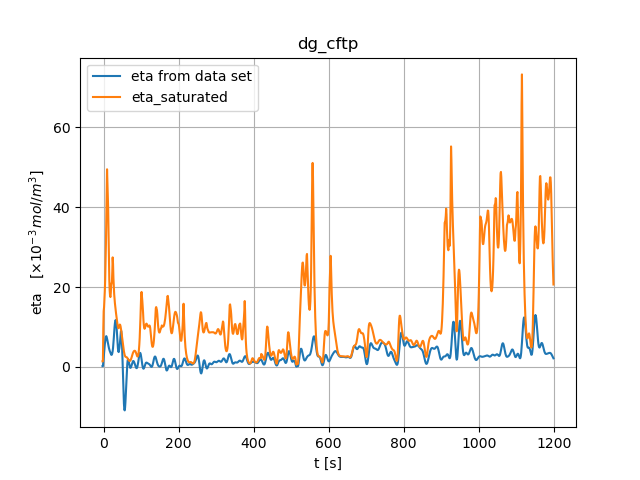
\includegraphics[width=\textwidth]{./figs/14_figs/bounded_eta_plots/eta_bounds_dg_cftp.png}
                \end{figure}
        \end{minipage}
        \begin{minipage}{0.49\textwidth}
                \begin{figure}[H]
                        \centering
                        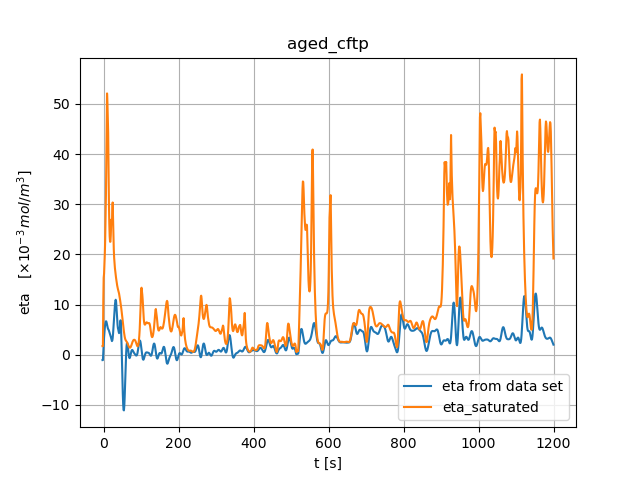
\includegraphics[width=\textwidth]{./figs/14_figs/bounded_eta_plots/eta_bounds_aged_cftp.png}
                \end{figure}
        \end{minipage}
        \caption{Saturated system response for cold FTP data}
\end{figure}

\begin{figure}[H]
        \begin{minipage}{0.49\textwidth}
                \begin{figure}[H]
                        \centering
                        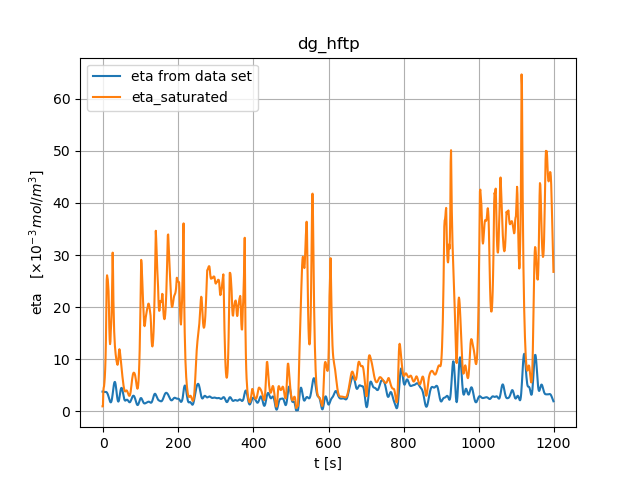
\includegraphics[width=\textwidth]{./figs/14_figs/bounded_eta_plots/eta_bounds_dg_hftp.png}
                \end{figure}
        \end{minipage}
        \begin{minipage}{0.49\textwidth}
                \begin{figure}[H]
                        \centering
                        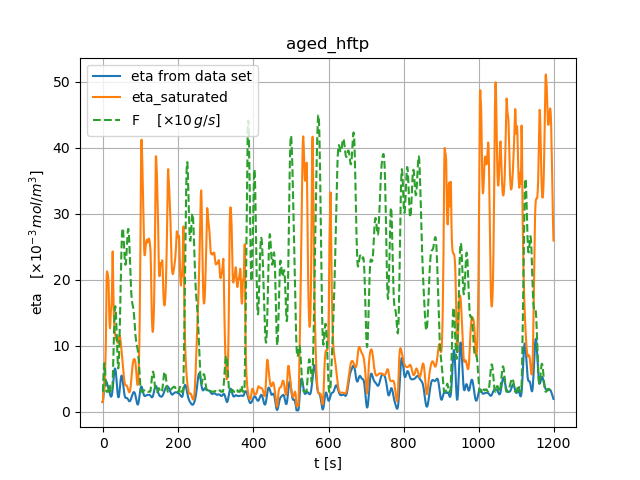
\includegraphics[width=\textwidth]{./figs/14_figs/bounded_eta_plots/eta_bounds_aged_hftp.png}
                \end{figure}
        \end{minipage}
        \caption{Saturated system response for hot FTP data}
\end{figure}

\begin{figure}[H]
        \begin{minipage}{0.49\textwidth}
                \begin{figure}[H]
                        \centering
                        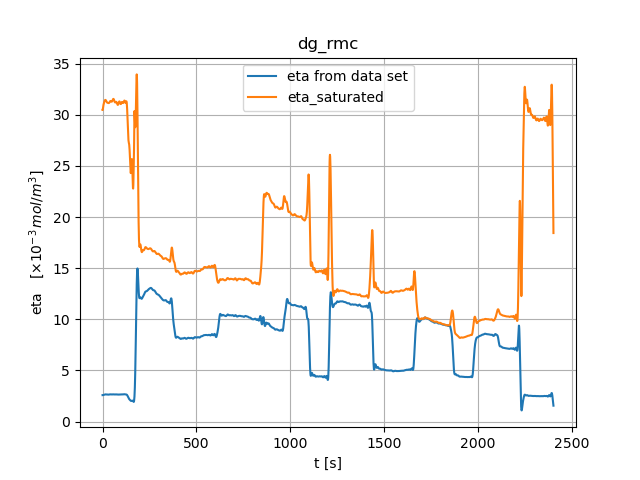
\includegraphics[width=\textwidth]{./figs/14_figs/bounded_eta_plots/eta_bounds_dg_rmc.png}
                \end{figure}
        \end{minipage}
        \begin{minipage}{0.49\textwidth}
                \begin{figure}[H]
                        \centering
                        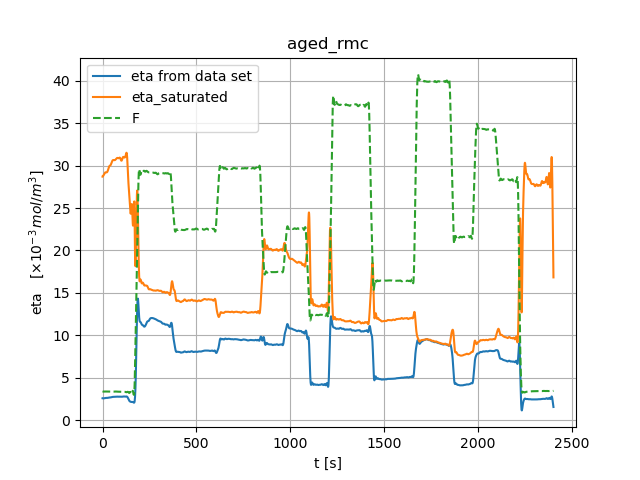
\includegraphics[width=\textwidth]{./figs/14_figs/bounded_eta_plots/eta_bounds_aged_rmc.png}
                \end{figure}
        \end{minipage}
        \caption{Saturated system response for RMC data}
\end{figure}

\subsection{Preliminary aging signature: Normalized maximum $NO_x$ reduction}

\begin{figure}[H]
        \begin{minipage}{0.49\textwidth}
                \begin{figure}[H]
                        \centering
                        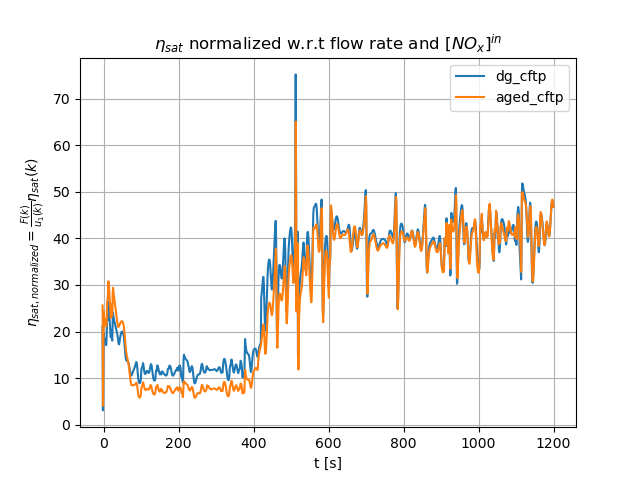
\includegraphics[width=\textwidth]{\froot/figs/14_figs/max_nox/max_nox_aged_cftp.png}
                \end{figure}
        \end{minipage}
        \begin{minipage}{0.49\textwidth}
                \begin{figure}[H]
                        \centering
                        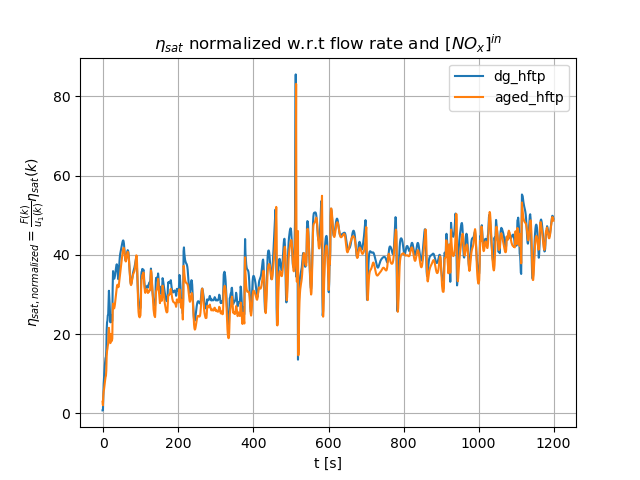
\includegraphics[width=\textwidth]{\froot/figs/14_figs/max_nox/max_nox_aged_hftp.png}
                \end{figure}
        \end{minipage}
        \caption{Maximum $NO_x$ reduction in FTP test data}
\end{figure}

\begin{figure}[H]
        \begin{minipage}{0.49\textwidth}
                \begin{figure}[H]
                        \centering
                        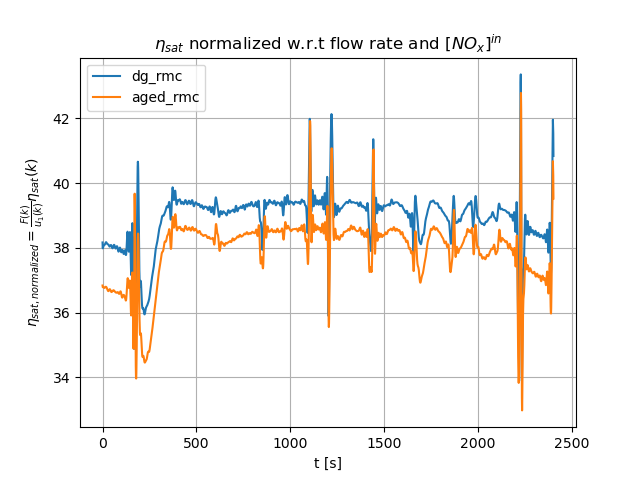
\includegraphics[width=\textwidth]{\froot/figs/14_figs/max_nox/max_nox_aged_rmc.png}
                        \caption{Maximum $NO_x$ reduction in RMC test data}
                \end{figure}
        \end{minipage}
        \begin{minipage}{0.49\textwidth}
                \begin{figure}[H]
                        \centering
                        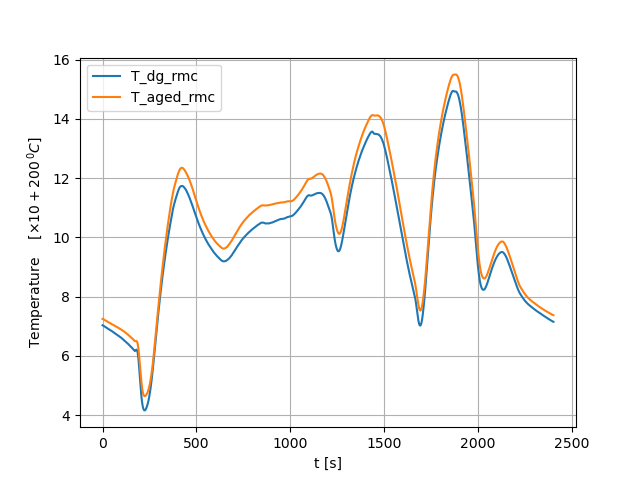
\includegraphics[width=\textwidth]{\froot/figs/14_figs/max_nox/max_nox_aged_rmc_T.png}
                        \caption{Temperature in RMC test data}
                \end{figure}
        \end{minipage}
\end{figure}

The plots demonstrate clearly the consistent difference between the aged and degreened catalysts. The maximum normalized $NO_x$ reduction is consistently higher for degreened catalyst than that of the aged.

